\definecolor{ublue}{rgb}{0.152,0.250,0.545}
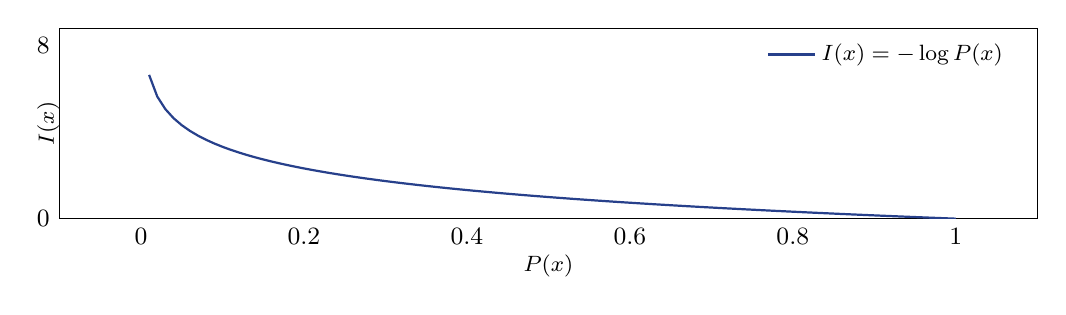
\begin{tikzpicture}
\begin{axis}[
  width=14cm,
  height=4cm,
  xlabel={{$\funp{P}(x)$}},
  ylabel={{$\funp{I}(x)$}},
  ylabel style={yshift=-1.5em,font=\footnotesize},
  xlabel style={yshift=0.3em,font=\footnotesize},
  xtick={0,0.2,...,1.0},
  ytick={0,8},
  y tick style={opacity=0},
  x tick style={opacity=0},
  domain=0.01:1,
  enlarge x limits=true,
  enlarge y limits={upper},
  legend style={draw=none,thick},
  xmin=0,
  xmax=1,
  ymin=0,
  ymax=8,
xticklabel style={font=\small}, %坐标轴字体大小
yticklabel style={font=\small}
]
\addplot[draw=ublue,samples=100,thick] {-log2(x)};
\legend{\footnotesize{$\funp{I}(x) = -\log \funp{P}(x)$}}
\end{axis}
\end{tikzpicture}

%---------------------------------------------------------------------